\documentclass[11pt]{article}
\usepackage{fullpage}
\usepackage{graphicx}
\graphicspath{ {images/} }
\title{CS63 Spring 2016\\Solving the Worlds Hardest Game}
\author{Vickram Rajendran, Ted Park}
\date{May 9 2016}
\usepackage[rightcaption]{sidecap}

\usepackage{wrapfig}

\begin{document}

\maketitle

\section{Introduction}

%Your paper should be 4-6 pages long.  In this section you should give
%a broad introduction to your project.  Assume that you are writing to
%an audience that is familiar with AI, but may not know the details of
%the particular technique that you are using.  You should give an
%overview of the approach being explored, and how you applied it to a
%particular problem.

In 2007, SnubbyLand released what they called "The World's Hardest Game" - a game geared towards gamers who believed that flash games were too easy and barely worth playing. The concept was simple. A player would control a small, red square and try to navigate through maze-like levels, acquiring coins without hitting the computer controlled blue balls. However, SnubbyLand created insanely difficult levels, requiring frame perfect inputs and complete mastery of the player's character in order to stumble their way through the levels. A running count of the deaths (number of encounters with the blue balls) were displayed on the screen, humbling players who thought they could easily beat the World's Hardest Game. The game was an instant success. Thousands of players tried and failed to beat the World's Hardest Game, and when people did beat the 30 levels, it was only with tens of hundreds of deaths. Our project was to create an Artificial Intelligence that would not only be able to play the World's Hardest Game, but conquer it completely without any deaths. The agent would have to take into account the locations of the blue enemies, and also be able to nimbly move through them - not an easy task by any means. 
\begin{figure}[h]
\centering

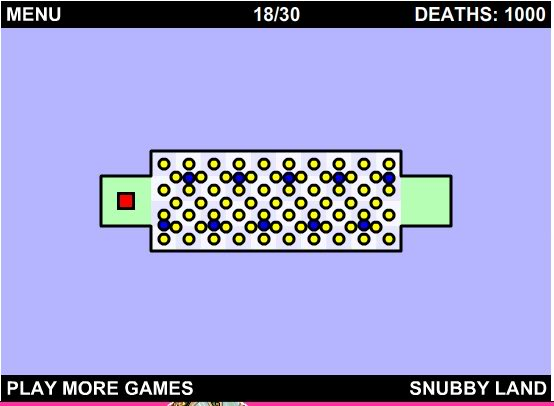
\includegraphics[scale = .5]{Hardgame4.jpg} \newline \newline
Figure 1: Playing the World's Hardest Game with an average amount of deaths.
\end{figure}

In order to accomplish such a task, we utilized reinforcement learning methods to allow the agent to focus on certain aspects of the level and find the best action to take at any given moment. In reinforcement learning algorithms, the agent is punished for doing wrong things (in this case, dying), and rewarded for doing the correct thing (getting the coins). Since the agent has incomplete information about the state of the game, as it does not know where the enemies may be, many reinforcement algorithms could not be used, so we used a version of Q-Learning, which is an algorithm that constantly updates the expected values of taking each action based on the rewards that one might achieve by taking that action. Approximate Q-Learning, the version used in this project, takes this a step further by allowing the agent to focus on certain features of the state of the game, like how many coins are left or if there are any enemies close to it. Our agent focused on the number of enemies one unit away from it in order to adequately dodge the enemies that could be coming for it. The agent can then "see" how these features are helping it win or lose the game, and weight how much it relies on each of these features correspondingly. Finally, after training on the level to determine how much it needs to rely on the features and to figure out which moves might be the best to take, the agent will then play on the level using its learned intelligence, and see how well it can handle the World's Hardest Game. 
\section{Method and Details}

%In this section you should explain how you implemented your project.
%Describe the data set used (number of patterns, number of features,
%escription of features, any preprocessing that was necessary) and its
%source.  You should provide all of the parameter settings used (such
%as learning rate, etc.).  You should also provide details about how
%the system was trained, and how you determined when to end training.

%Details about how to test and run your code should not be given in the
%paper, but should instead be described in the README file in the lab
%directory. 
In order to develop and test the agent, we first needed to create our own environment of the World's Hardest Game in Python, which involved creating a player controlled character, and enemies with computer controlled movement, as well as determining win conditions and the legal moves possible, all while finding ways to display this to the user. To accomplish this in a timely fashion, we attempted to modify existing code to create this environment. The University of California, Berkeley developed an open source Pacman AI project, complete with user-interface and display which we have used previously in other labs (Lab 07). Still, while this gave an adequate baseline to work from, Pacman is nothing like the Worlds Hardest Game. We first had to create entirely new assets, such as removing Pacman and replacing it with the red square of the World's Hardest Game, and then also removing the assets of the ghosts and replacing them with the blue dots of the Worlds Hardest Game. Modifying these values also required us to modify the animation and movement methods that UC, Berkeley used in order to deal with collision cases and hitboxes. Once this was done, we then needed to create entirely new behavior for the enemies. Currently they were following the ghosts behavior, which is seemingly random and nothing like the behavior of the enemies in the World's Hardest Game. Each of the enemies had to be individually coded in our implementation of the World's Hardest Game, as we created them to move between specific areas, just like the actual game has them.

After the movement of the enemies was finished, we then had to create entirely new layouts in order to represent the levels of the game, and so we had to figure out which levels were the best representations of the game to look at. Each of the levels chosen test different portions of the Agent's learning. Our level 1 mirrors the first level of the original World's Hardest Game, and it attempts to discover if the Agent understands the basic principle of the game - to win the game by getting all of the coins and dodging the agents. Our level 2 mirrors the eighteenth level of the original game, and it tests whether the Agent is dexterous enough to nimbly move through a large amount of enemies to get the coins. Similarly, Level 3 tests if the Agent will take the hardest, but shortest path or the easy and long path. Level 4 tests if the Agent can find the right time in order to go through narrow paths, and level 5 tests if the Agent can think ahead and stop itself from accidentally reaching a no-win scenario where it is surrounded by enemies or is unable to move anywhere without dying. \newline
\begin{figure}[t]
\centering

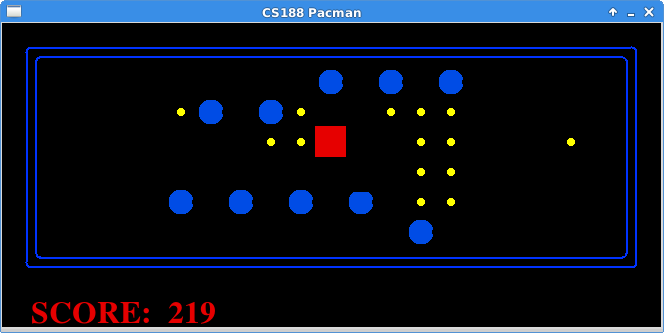
\includegraphics[scale = .5]{WHGL2.png} \newline \newline
Figure 2: Agent solving Level 2 in our implementation of the World's Hardest Game
\end{figure}
Finally, we had to make all of these changes so that it was compatible with the  Approximate Q-Agent we wrote in a previous lab. After making slight modifications to this code so that everything worked, we changed the features that the Agent would be looking for, making it so that it just looks at enemies that were one step away and the amount of coins left, along with a bias factor. We trained the agent on each of these levels 10, 30, and 50 times, and then tested to see how many times it died when attempting the level ten times. 
\section{Results}

%In this section you should show and analyze the results.  Measure the
%performance of your system, and if possible compare your performance
%to other implementations. Use tables and figures to illustrate the
%results.  If you can't fit all of the pictures that you'd like to show
%in the paper, you can make an accompanying web page and point the
%reader to it.

%Even if your project is not as successful as you'd hoped, you still
%need to show results.  This section is one of the key parts of any
%scientific paper.  Be sure to provide adequate information so that the
%reader can evaluate the outcomes of your experiments. 
The results can be summarized in the following figure. 


\begin{center}
 \begin{tabular}{||c c||} 
 \hline
 Level & Wins (/10) \\ [0.5ex] 
 \hline\hline
 1 & 10 \\ 
 \hline
 2 & 10 \\ 
 \hline
 3 & 10 \\ 
 \hline
 4 & 0 \\ 
 \hline
 5 & 0 \\ 
 \hline
\end{tabular} \newline \newline
Figure 3: Results of the training of the Agent on each of the Levels. 
\end{center}

There are many interesting things to note about these results. Firstly, the number of training episodes did not seem to matter at all once the agent had at least 10 training episodes. Regardless of the amount of training, the agent would either completely decimate the level, having no trouble whatsoever, or the agent would completely fail and be unable to solve the level with even 100 training episodes. This can be reasonably explained by attempting to figure out why the agent failed so immensely on levels 4 and 5.
\begin{figure}[t]
\centering

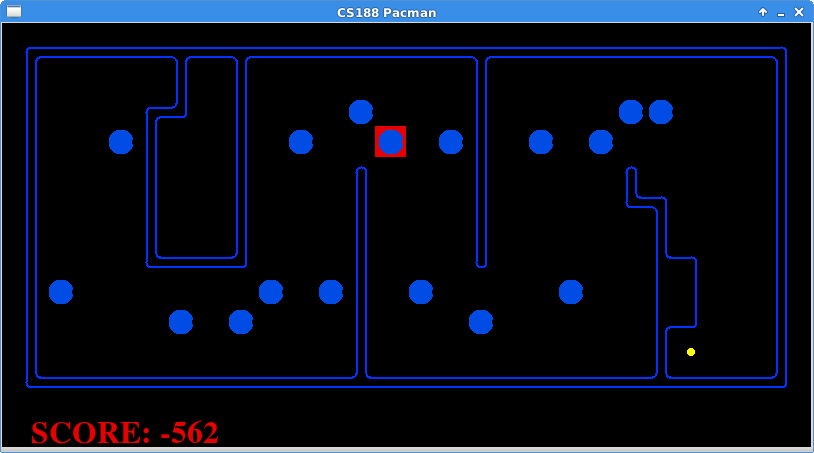
\includegraphics[scale = .5]{WHGL4.png} \newline \newline
Figure 4: The Agent never got past this portion of level 4.
\end{figure}

The reason that the agent fails so heavily on this portion of the level is that it cannot see more than one enemy in advance. Recall that the features that were selected for the Approximate Q-Agent were the number of enemies one step away - when the agent is two steps to the left of the state shown in Figure 4, it is merely trying to determine how to make it to the right. However, once it gets there, it realizes that it is in a dead end since it did not notice the blue ball coming from below that is now directly adjacent to it, and it cannot stay where it is since otherwise it would die. The correct option would be to wait until the ball two steps away is far away before moving, but the agent cannot detect that, and the agent thus dies before it can find a different way around this. 

Some ways to get around this would be to facilitate some random movement, but this could be completely disastrous since it would have to randomly decide to wait in one area longer in certain cases, which is pretty unlikely behavior for the agent to learn. The better change would be to adjust the features that the agent is learning on, and try to have it learn on more things, such as the direction that the balls are currently going relative to which direction it wants to go, and also the balls that would meet up with it if it continues on the path that it is going on. This would allow the agent to make some decisions about future actions, instead of just thinking about the next action that it will take. Another method, though much harder to implement, would be an online Monte Carlo simulation type of algorithm that constantly does simulations and determines how to get past stumbling blocks it might hit in the future. This would be likely be the most prolific and general solution, but it would also be the hardest to implement, as creating a simulation for such complex game behavior is certainly nontrivial, especially since the branching factor is so high in such a game. This is also the same reason it failed on level 5 - it could not detect the dead end it was traveling into until it was too late. 
\begin{figure}[t]
\centering

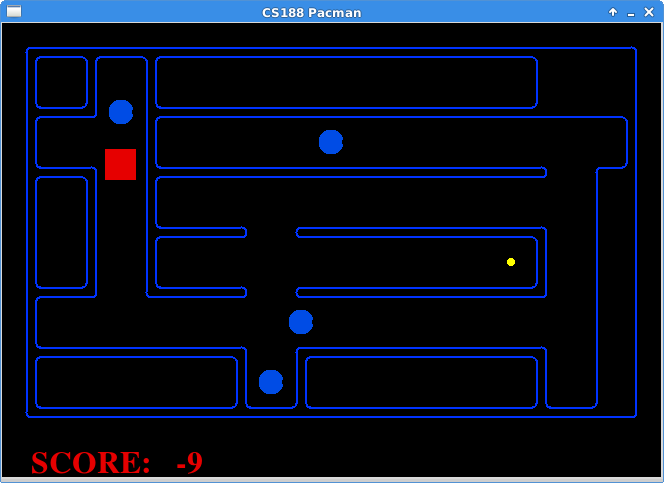
\includegraphics[scale = .4]{WHGL5.png} \newline \newline
Figure 5: The Agent is unaware that it has already lost on Level 5. 
\end{figure}

\section{Conclusions}

%This section should sum up what you did and what you found. 
After modifying UC, Berkeley's open-source Pacman interface and code, along with implementing an Approximate Q-Learning Agent, we were able to create an interface for the World's Hardest Game and test how well reinforcement learning algorithms worked on the World's Hardest Game. We discovered that levels that tested how fast or accurate the player could use their character were trivial for our AI, and only through larger mindgames was the game able to beat our agent at some of the levels. We also discovered that very few episodes of training were required in order for the agent to perform perfectly, showing that this agent is very efficient. Though our agent certainly has many areas to improve upon, it performed exceedingly well in certain scenarios. The fact that it required very little training in order to perform so well is also heartening - only ten episodes were required to completely solve three of the harder levels in the World's Hardest Game. Our results show that applying Approximate Q-Learning Algorithms to agents in order to solve the World's Hardest Game certainly dominates some of the levels, but more work will be necessary in order to create the prolific agent that would be able to solve all of the levels without dying. As noted in the Results section of the paper, the main issue with the current agent is the fact that it cannot detect when it accidentally goes into a losing scenario before it is too late for it to remove itself from the scenario. There are many different avenues for further experimentation in the Approximate Q-Learning viewpoint, and there are also possibilities to apply Monte-Carlo and simulation methods to get an even better algorithm. Also, it is important to note that this type of algorithm could be easily generalized to other games as well - Approximate Q-Learning certainly worked on Pacman, and was able to be modified to work on the World's Hardest Game as well, so it is only natural that slight modifications of our interface and algorithm could allow this to work on other popular puzzle games such as "bloxorz", or "2048". Regardless of the poor performance of our agent on some levels, it clearly shows a proof of concept, making a clear statement that what might be the World's Hardest Game for humans is trivial for an Artificial Intelligence. 

\end{document}